\documentclass{article}

\usepackage{amsmath, amsthm, amssymb, amsfonts, mathtools,enumitem, stmaryrd}
\usepackage{tikz-cd}
\usepackage{graphicx}
\usepackage{float}
\usepackage{booktabs}
\usepackage{tocbasic}
\usepackage{geometry}
    \geometry{
        a4paper,
        left = 40mm,
        top = 20mm,
        right = 40mm,
        bottom = 30mm
    }
\setlength{\parindent}{0pt}

\theoremstyle{definition}
\newtheorem{problem}{Problem}
\newtheorem{solution}{Solution}
\newtheorem*{example}{Example}
\newtheorem*{exercise}{Exercise}
\newtheorem*{definition}{Definition}
\newtheorem{theorem}{Theorem}[section]
\newtheorem*{theorem*}{Theorem}
\newtheorem{proposition}[theorem]{Proposition}
\newtheorem*{proposition*}{Proposition}
\newtheorem{lemma}[theorem]{Lemma}
\newtheorem*{lemma*}{Lemma}
\newtheorem{corollary}[theorem]{Corollary}
\newtheorem*{corollary*}{Corollary}
\newtheorem*{remark}{Remark}
\newtheorem*{construction}{Construction}

\newcommand{\Frac}{\operatorname{Frac}}
\newcommand{\im}{\operatorname{im}}
\newcommand{\acts}{\circlearrowright}
\newcommand{\rank}{\operatorname{rank}}
\newcommand{\End}{\operatorname{End}}
\newcommand{\Hom}{\operatorname{Hom}}
\newcommand{\Char}{\operatorname{char}}
\newcommand{\Tr}{\operatorname{Tr}}
\renewcommand{\span}{\operatorname{span}}
\newcommand{\ad}{\operatorname{ad}}

\title{Number Theory Reading Group}
\author{Thanic Nur Samin}
\date{\vspace{-5ex}}

\begin{document}

\maketitle

\tableofcontents

\section{Thursday, 9/12/2024, Representation of \(\mathfrak{sl}_2(\mathbb{F})\) by Hechi}

\[
    \mathfrak{sl}_2(\mathbb{F}) \coloneqq \{ g \in \mathfrak{gl}_2(\mathbb{F}) \mid \Tr(g) = 0 \}
\]

We assume \(\Char(\mathbb{F}) = 0\) and \(\mathbb{F}\) is algebraically closed.

\begin{theorem}
    \(\mathfrak{sl}_2(\mathbb{F})\) is semisimple
\end{theorem}

\begin{proof}
    Direct computation of the Killing Form.
\end{proof}

Recall: if \(\mathfrak{L}\) is semisimple and \(\phi: \mathfrak{L}  \to \mathfrak{gl}(V)\) is a representation.

\(\mathfrak{L} \ni x = s+n\) abstract jordan decomposition.

\(\implies \phi(x) = \phi(s) + \phi(n)\) is the Jordan decomposition of \(\phi(x)\) in \(\phi(\mathfrak{L})\).

From now on, \(\mathfrak{L} = \mathfrak{sl}_2(\mathbb{F}) = \mathfrak{sl}(2,\mathbb{F})\).

\((V,\phi)\) is a representation.

Basis of \(\mathfrak{L}\):

\[
    x = \begin{bmatrix}
        0 &  1 \\
        0 &  0 \\
    \end{bmatrix}
\]

\[
    y = \begin{bmatrix}
        0 &  0 \\
        1 &  0 \\
    \end{bmatrix}
\]

\[
    h = \begin{bmatrix}
        1 &  0 \\
        0 &  -1 \\
    \end{bmatrix}
\]

Thus we have \([h,x] = 2x, [h,y]=-2y, [x,y]=h\). 

Since \(h\) is diagonal, \(h\) is semisimple.

\(\implies \phi(h)\) is semisimple and thus diagonalizeable. \(\in \End(V)\). 

We can decompose \(V = \bigoplus_{\lambda} V_\lambda\) where \(V_\lambda = \{ v\in V \mid h v = \lambda v \} \) for all \(\lambda \in \mathbb{F}\). 

We say \(V_\lambda\) is a \underline{weight space} with \(\lambda\) as its weight.

\begin{lemma}
    [7.1] Suppose \(v\in V_\lambda\). Then,

    \begin{enumerate}[label=\arabic*)]
        \item \(xv \in V_{\lambda+2}\)
        \item \(yv \in V_{\lambda-2}\) 
    \end{enumerate} 
\end{lemma}

\begin{proof}
    \begin{enumerate}[label=\arabic*)]
        \item \(h(xv) = [h,x]v + x(hv) = 2xv + \lambda xv = (\lambda + 2)xv\)
        \item \(h(yv) = [h,y]v + y(hv) = -2yv + \lambda yv = (\lambda - 2)yv\)  
    \end{enumerate} 
\end{proof}

\begin{center}
    \begin{tikzcd}
        V_{\lambda-2} & V_{\lambda} \ar[l, bend left, "y", swap] \ar[r, bend right, "x", swap] \ar[loop, "h", swap] & V_{\lambda+2}
    \end{tikzcd}
\end{center}

Note that \(\div V < \infty\)

Thus, \(\exists v \in V\) such that \(x\cdot v = 0\).

Such a \(v\) is called a \underline{maximal vector}. 

For now, assume \(V\) is irreducible.

Let \(v_0\) be a maximal vector with weight \(\lambda\).

\begin{definition}
    For \(i > 0\) integer, \(v_i = \frac{y^i\cdot v_0}{i!}\) 

    Also, \(v_{-1}=0\).
\end{definition}

\begin{lemma}
    [7.2]

    \begin{enumerate}[label=\arabic*)]
        \item \(h\cdot v_i = (\lambda - 2i)v_i\) 
        \item \(y\cdot v_i = (i+1)v_{i+1}\)
        \item \(x\cdot v_i = (\lambda - i + 1) v_{i-1}\)  
    \end{enumerate} 
\end{lemma}

\begin{proof}
    \begin{enumerate}[label=\arabic*)]
        \item We use induction. Base case is clear.
        
        Assume it is true for \(i-1\). 

        \(v_{i-1} \in V_{\lambda - 2(i-1)}\) 

        Thus, \(v_i = \frac{1}{i} \cdot y v_{i-1}\)
        
        Lemma 7.1 implies \(v_i \in V_{\lambda - 2i}\).

        \item \(y\cdot v_i = (i+1) v_{i+1}\) by definition of \(v_i\). 
        
        \item \(i x\cdot v_i = x (yv_{i-1}) = [x,y]v_{i-1} + yx v_{i-1} = h v_{i-1} + y x v_{i-1} = (\lambda - 2(i-1))v_{i-1} + (\lambda -i + 2)y v_{i-2} = i(\lambda -i + 1)v_{i-1}\) 
    \end{enumerate} 
\end{proof}

\(\dim V < \infty\) so it must end at some point.

So, at some point, it'll become \(0\). \(v_0, \cdots ,v_m \neq 0, v_{m+1} = 0\).

\begin{definition}
    \(m\) is the integer so that \(v_m \neq 0, v_{m+1} = 0\).
\end{definition}

By Lemma 7.2,

\(\span \{v_0, \cdots , v_m\}\) is a sub-representation of \(V\).

Since \(V\) is irreducible,

\(V = \span \{v_0, \cdots , v_m\}\) 

\underline{Note}: by 7.2(3),

\(0 = x \cdot v_{m+1} = (\lambda - m) v_m\) 

Since \(v_m \neq 0\) we have \(\lambda = m\).

Thus, \(\dim V = m+1 = \lambda + 1\)

Here \(m\) is the \underline{highest weight}. 

\[
    V = V_{-m} \oplus V_{-m + 2} \oplus \cdots \oplus V_{m-2} \oplus V_m
\]

\begin{construction}
    Suppose \(L \curvearrowright \mathbb{F}[X,Y]\) [as a \(\mathbb{F}\)-space].
    
    \(\rho (x) = X \frac{\partial}{\partial Y} \) 

    \(\rho (y) = Y \frac{\partial}{\partial X} \)
    
    \(\rho (h) = x \frac{\partial}{\partial x} - y \frac{\partial}{\partial y}\)
    
    Consider subrepresentations \(\mathbb{F} [X,Y]_m\) [symmetric polynomials of degree \(m\), dimension \(m+1\)].

    \begin{center}
        \begin{tikzcd}
            0 & X^m \ar[l, bend left, "x", swap] \ar[r, bend right, "y", swap] \ar[loop, "h", swap] & X^{m-1}Y & \cdots
        \end{tikzcd}
    \end{center}

\end{construction}

\newpage

\section{Thursday, 9/19/2024, Representation of \(\mathfrak{sl}_2(\mathbb{F})\) by Hechi}

\subsection*{Root Space Decomposition}

Let \(\mathcal{L}\) be a non-zero semisimple lie algebra over \(\mathbb{F}\) with \(\Char \mathbb{F} = 0\) and \(\mathbb{F}\) algebraically closed.

\begin{definition}[Toral Subalgebra]
    A subalgebra \(\mathcal{H} \subseteq \mathcal{L}\) \underline{toral} if it consists of semisimple elements.
\end{definition}

\begin{remark}
    If every element in \(\mathcal{L}\) is ad-nilpotent, then by Engel's Theorem \(\mathcal{L}\) is nilpotent. Thus it is not semisimple. 

    So, there exists a non-zero toral subalgebra.
\end{remark}

Fix \(\mathcal{H}\) to be the \underline{maximal toral subalgebra}. A maximal subalgebra exists since \(\mathcal{L}\) is finite dimensional.

\begin{lemma}
    [8.1] A toral subalgebra \(\mathcal{T}\) is abelian.
\end{lemma}

\begin{proof}
    Suppose \(x\in \mathcal{T}\). We will prove that \(\ad_{\mathcal{T}}x = 0\) [as a map].

    \(\ad_T x\) is diagonalizeable. Assume some eigenvalue is non-zero. Then, we can find eigenvactor \(y\in T\) with eigenvalue \(a \neq 0\). So, \([x,y]=ay\).

    Now, \(\ad_T y (x) = [y,x] = -ay\). Since \([y,y]=0\) we see that \(-ay\) is an eigenvector of \(\ad_T y\) with eigenvalue \(0\). 

    \(\ad_T y\) is also diagonalizeable. Suppose \(v_1, \cdots , v_n\) is the eigenbasis of \(\ad_T y\) with eigenvalues \(\lambda_1, \cdots , \lambda_n\). Then \(x = a_1 v_1 + \cdots + a_n v_n\) for \(a_i \in \mathbb{F} \).

    WLOG, \(v_1 = y\).

    \[
        [y,x] = a_1 \lambda _1 v_1 + \cdots + a_n \lambda_n v_n = -ay
    \]

    By comparing coefficients, \(a_1 \lambda _1 = -a\). But \(\lambda_1 = 0\). This is a contradiction. 

\end{proof}

Now, we fix \(\mathcal{H}\) to be a maximal toral subalgebra. It is not necessarily unique.

Note that \(\ad H\) is a \underline{commuting family} in \(\End(\mathcal{L})\). From linear algebra we know that \(\ad H\) is \underline{simultaneously diagonalizeable}.

\begin{definition}
    [Root Space Decomposition]
    Suppose \(\mathcal{H} ^{\ast} \) is the dual space of \(\mathcal{H}\). We can write:

    \[
        \mathcal{L} = \bigoplus_{\alpha \in H^{\ast}} \{ x \in \mathcal{L} \mid [h,x] = \alpha (h) x \forall h\in H \}
    \]

    \[
        = \mathcal{L}_0 \oplus \bigoplus_{\alpha \in \Phi} \mathcal{L} \alpha 
    \]

    where \(\Phi = \{ \alpha \in H^{\ast} \setminus \{ 0 \}  \mid  \mathcal{L} \alpha \neq 0\} \) and \(\mathcal{L} _0 = C_{\mathcal{L}}(\mathcal{H})\) [the centralizer]. 

    This is called the \underline{root space decomposition}. 

\end{definition}

\begin{example}
    \(\mathfrak{sl}_2(\mathbb{F})\) has basis:

    \[
        x = \begin{bmatrix}
            0 &  1 \\
            0 &  0 \\
        \end{bmatrix}, y = \begin{bmatrix}
            0 &  0 \\
            1 &  0 \\
        \end{bmatrix}, h = \begin{bmatrix}
            1 &  0 \\
            0 &  -1 \\
        \end{bmatrix}
    \]

    Then the root space decomposition is:

    \[
        \mathfrak{sl}_2(\mathbb{F}) = \mathcal{H} \oplus \mathcal{L}_{-2} \oplus \mathcal{L}_{2}
    \]

    \(\mathcal{L}_{-2}\) contains the linear form sending \(h\) to \(-2\). 

\end{example}

\begin{proposition}
    [8.1] Let \(\alpha , \beta \in \mathcal{H} ^{\ast}\). Then,

    \begin{enumerate}[label=\arabic*)]
        \item \([L_\alpha , L_\beta] \subseteq L_{\alpha + \beta}\) [by Jacobi Identity]
        \item \(\alpha \neq 0 \implies \forall x\in L_\alpha\) is nilpotent [by 1]
        \item \(\alpha + \beta \neq 0 \implies L_\alpha \perp L_\beta\) w.r.t.\ the \underline{Killing Form}. 
    \end{enumerate} 
\end{proposition}

\begin{proof}
    [Proof of 3] Find \(h\in \mathcal{H}\) such that \((\alpha + \beta)(h) \neq 0\). Then,

    \[
        \kappa([h,x],y) = - \kappa([x,h],y) = - \kappa(x,[h,y])
    \]

    \[
        \implies (\alpha+\beta)(h)\kappa(x,y) = 0
    \]
\end{proof}

In particular, \(L_0 \perp L_\alpha\) when \(\alpha \in \Phi\). 

\begin{corollary}[8.1]
    The Killing Form restricted to \(\mathcal{L}_0\), \(\kappa|_{\mathcal{L}_0}\) is non-degenerate. 
\end{corollary}

\begin{proposition}
    [8.2] \(\mathcal{H} = \mathcal{L}_0 = C_{\mathcal{L}}(\mathcal{H})\).
\end{proposition}

\begin{proof}
    Tedious linear algebra
\end{proof}

\begin{corollary}
    [8.2] The Killing Form restricted to \(\mathcal{H}\), \(\kappa |_{\mathcal{H}}\) is non-degenerate.
\end{corollary}

This implies, the map \(H \to H^{\ast}\) given by \(x \mapsto \kappa (x,-)\) is an \underline{isomorphism}.

For each \(\phi \in \mathcal{H} ^{\ast}\) we can define \(t_{\phi} \in \mathcal{H} \) to be the pre-image of this isomorphism. So it satisfies

\[
    \phi(h) = \kappa (t_{\phi}, h) \quad \forall h\in \mathcal{H}
\]

\begin{proposition}
    [8.3]

    \begin{enumerate}[label=\arabic*)]
        \item \(\Phi\) spans \(\mathcal{H} ^{\ast}\) 
        \item If \(\alpha \in \Phi\) then \(-\alpha \in \Phi\)
        \item \(x\in \mathcal{L}_\alpha, y\in \mathcal{L}_{-\alpha} \implies [x,y] = \kappa (x,y)t_\alpha\)
        \item \(\alpha(t_\alpha) = \kappa (t_\alpha , t_\alpha) \neq 0\) 
        \item \(\dim [\mathcal{L}_\alpha, \mathcal{L}_{-\alpha}] = 1\), spanned by \(t_\alpha\)  
        \item Pick any non-zero \(x_\alpha\in L_\alpha \setminus \{ 0 \}\). Then there exists \(y_\alpha \in \mathcal{L}_{-\alpha}\) such that \(x_\alpha , y_\alpha , h_\alpha \coloneqq [x_\alpha , y_\alpha]\) spans a subalgebra isomorphic to \(\mathfrak{sl}_2(\mathbb{F})\), with the isomorphism \(x_\alpha \mapsto x, y_\alpha \mapsto y, h_\alpha \mapsto h\) 
        \item \(h_\alpha = \frac{2 t_\alpha}{\kappa (t_\alpha , t_\alpha )}\).  
    \end{enumerate} 
\end{proposition}

If \(V\) is a \(\mathfrak{sl}_2(\mathbb{F})\)-module, recalling that \(h = \begin{bmatrix}
    1 &  0 \\
    0 &  -1 \\
\end{bmatrix}\),

\[
    V = \bigoplus_{\lambda \in \mathbb{F}} V_\lambda \text{ eigenspaces of } h
\]

Recall that all \(\mathfrak{sl}_2(\mathbb{F})\)-module is of the form:

\[
    \mathfrak{sl}_2(\mathbb{F}) \curvearrowright \mathbb{F} [X,Y]
\]

\[
    \rho (x) = X \frac{\mathrm{d}}{\mathrm{d}Y}, \rho (y) = Y \frac{\mathrm{d}}{\mathrm{d}X} , \rho (h) = X \frac{\mathrm{d}}{\mathrm{d}X} - Y \frac{\mathrm{d}}{\mathrm{d}Y}  
\]

and \(V = \mathbb{F} [X,Y]_m\) [homogeneous polynomials of degree \(m\)] is irreducible and give us all irreducible representations. 

Then we have:

\[
    V = V_{-m} \oplus V_{-m + 2} \oplus \cdots \oplus V_{m-2} \oplus V_{m}
\]

Where \(V_m\) is generated by \(X^m\) and \(V_{-m}\) is generated by \(Y^m\) 

\begin{center}
    \begin{tikzcd}
        Y^m \ar[r, bend right, "x", swap] & X Y^{m-1} \ar[l, bend right, "y", swap] \ar[loop, "h", swap] & \cdots & X^m
    \end{tikzcd}
\end{center}

If \(m\) even, \(0 \neq V_0 \subseteq V\)

If \(m\) odd, \(0 \neq V_1 \subseteq V\)

\begin{corollary}
    \(V\) is a \(\mathfrak{sl}_2(\mathbb{F})\)-module. Then \(\dim V_0 + \dim V\) gives the number of summands in the irreducible decomposition of \(V\).
\end{corollary}

Consider \(\mathcal{S}_\alpha = \span\{ x_\alpha , y_\alpha , h_\alpha  \} \cong \mathfrak{sl}_2(\mathbb{F})\) and its adjoint representation (\(\mathcal{L}\) is an \(\mathcal{S}_\alpha\) module).

Fix \(\alpha \in \Phi \) and let \(\mathcal{M} = \mathcal{H} + \sum_{c\in \mathbb{F} ^\times } \mathcal{L}_{c \alpha}\). 

By proposition 8.1, \(\mathcal{M}\) is a submodule of \(\mathcal{L}\) [since \([\mathcal{L}_{c_1 \alpha}, \mathcal{L}_{c_2 \alpha}] \subseteq \mathcal{L}_{(c_1 + c_2)\alpha}\)].

If \(0 \neq x \in \mathcal{L}_{c \alpha}\) we see that \([h_\alpha , x] = c \alpha (h_\alpha)\cdot x = 2 c x\) 

\(\implies\) \(2c\in \mathbb{Z}\) and a \(\underbrace{\text{weight}}_{\text{eigenvalue}}\) of \(h_\alpha\) is \(0\) or an integer multiple of \(\frac{1}{2}\).

Then \(\mathcal{M} = \underbrace{\ker \alpha}_{\text{vectors of weight } 0} + \underbrace{\mathbb{F} \cdot h_\alpha}_{\text{weight } 0, \pm 2}\) 

Therefore, \(\mathcal{M}\) contains vectors of weight only \(0\) or \(\pm 2\). 

Therefore, if \(\alpha \in \Phi\) we have \(c = \pm 1\).

\(\mathcal{M} = \mathcal{H} + \mathcal{S}_\alpha\). Suppose \(h_\alpha ^c \) is the complement of \(h_\alpha\) in \(\mathcal{H} \). 

Then, \(\mathcal{H} + \mathcal{S}_\alpha = \underbrace{h_\alpha^c}_{\text{abelian}} + \underbrace{\mathcal{S}_\alpha}_{\text{irreducible}}\) has \(\dim \mathcal{H} - 1 + 1 = \dim \mathcal{H} = \dim \mathcal{M} - 2\) irreducible summands.

On the other hand, the number of irreducible summands of \(\mathcal{M}\) is \(\underbrace{\dim \mathcal{M}_0}_{\dim \mathcal{M} - 2} + \underbrace{\dim \mathcal{M}_1}_{0}\) 

Therefore, \(\mathcal{H} + \mathcal{S}_\alpha \subseteq \mathcal{M}\) must be \underline{equal}.

Therefore, \(\dim \mathcal{L}_\alpha = 1\).

Now, suppose \(\beta \neq \pm \alpha \in \Phi\). Then, \(\exists r,q\) such that \(\beta - r \alpha , \beta - (r-1)\alpha , \cdots , \beta + q \alpha\) are roots and outside outside these, i.e.\ \(\beta - (r+1)\alpha , \beta + (q+1)\alpha\) are not.

To see this, suppose \(K = \sum_{i\in \mathbb{Z}}^{} \mathcal{L}_{\beta + i \alpha} \subseteq \mathcal{L}\) is a \(\mathcal{S}_\alpha\)-submodule. We know that \(\beta + i \alpha \neq 0\).

Weights:

\[
    \beta(h_\alpha) + i \alpha (h_\alpha) = \beta (h_\alpha) + 2i
\]  

So, weights are either all even or all odd.

Therefore, \(K\) is irreducible.

Consider \(\gamma , \delta \in \mathcal{H} ^{\ast}\).

Define \((\gamma , \delta) = \kappa (t_\gamma , t_\delta)\) on \(E_\mathbb{Q} = \span_\mathbb{Q} (\Phi)\) then \((\cdot,\cdot)\) extends to \(E = E_\mathbb{Q} \otimes _\mathbb{Q} \mathbb{R} \) is positive definite.

Then \(E\) is an Euclidean Space.

\[
    (\Phi, E) \text{ is called a \underline{root system}}.
\]

\newpage

\section{Thursday, 9/26/2024, Root Systems by Zoia}

Let \(E\) be an euclidean space. Suppose \((\alpha ,\beta)\) is a symmetric bilinear form on \(E\).

Reflection in \(E\) fixes some hyperplane \(H\). If \(\alpha\) is perpendicular to \(H\) then the reflection sends \(\alpha\) to \(-\alpha\) 

Consider \(\alpha \in E\) and \(P_\alpha = \{ \beta \in E \mid (\alpha , \beta) = 0 \} \) the hyperplane perpendicular to \(\alpha\). Suppose \(\sigma_\alpha\) is the reflection w.r.t.\ this hyperplane. Then,

\[
    \operatorname{proj}_\alpha (\beta) = \frac{(\beta , \alpha)}{(\alpha , \alpha)}\alpha 
\]

\[
    \sigma_\alpha (\beta) = \beta - 2 \operatorname{proj}_\alpha(\beta) = \beta - 2\frac{(\beta,\alpha)}{(\alpha ,\alpha)}\alpha
\]

Define:

\[
    \langle \beta , \alpha  \rangle = 2 \frac{(\beta,\alpha)}{(\alpha,\alpha)}
\]

Note that \(\langle \beta ,\alpha  \rangle \) is linear only in \(\beta \). Then, 

\[
    \sigma_\alpha (\beta) = \beta - \langle \beta ,\alpha  \rangle \alpha 
\]

\begin{lemma}
    Let \(\Phi\) be a finite subset of \(E\) so that \(\Phi\) spans \(E\). Suppose all reflections \(\sigma_\alpha (\alpha \in \Phi)\) leaves \(\Phi\) invariant. If \(\sigma\in \operatorname{GL}(E)\) fixes hyperplane \(P\) of \(E\) and sends \(0 \neq \alpha \in \Phi\) to \(-\alpha\), then \(\sigma = \sigma_\alpha\) and \(P = P_\alpha\).
\end{lemma}

\begin{proof}
    Suppose \(\tau = \sigma \sigma_\alpha = \sigma \sigma _\alpha ^{-1} \).

    Then, \(\tau(\Phi) = \Phi , \tau (\alpha ) = \alpha\) and \(\tau\) acts as \(\operatorname{id}\) on \(\mathbb{R} \cdot \alpha\) and \(E / R\cdot \alpha\) eigenvalues are \(1\). So we have \((T-1)^L\) where \(L = \dim E\).
    
    \(\beta , \tau (\beta), \dots \tau^k(\beta)\) \(\exists k\) that fixes all \(\beta \in \Phi \) 

    \(\Phi\) spans \(E\), so \(\tau ^ k = 1\). So \(T^k - 1 = 0\).

    If \(m(T)\) is the minimal polynomial of \(\tau\), then:

    \[
        m(T) \mid T^k - 1
    \]

    \[
        m(T) \mid (T-1)^k
    \]

    Therefore, \(m(T) = T - 1\).
    
    Therefore, \(\tau = \operatorname{id}\).

    Thus \(\sigma \sigma_\alpha ^{-1} = \operatorname{id} \implies \sigma = \sigma_\alpha \) 
\end{proof}

\begin{definition}
    [Root Systems]

    A finite subset \(\Phi\) of \(E\) is a root system in \(E\) if:

    \begin{enumerate}[label=\arabic*R)]
        \item \(\Phi\) spans \(E\), does not contain \(0\).
        \item If \(\alpha \in \Phi\) then only multiples of \(\alpha\) in \(\Phi\) are \(\pm \alpha\).
        \item If \(\alpha \in \Phi\), then \(\sigma_\alpha\) leaves \(\Phi\) invariant. \([\forall \beta \in \Phi, \sigma_\alpha (\beta)\in \Phi ]\) 
        \item If \(\alpha ,\beta \in \Phi \) then \(\langle \beta , \alpha  \rangle \in \mathbb{Z} \). \(\left[ \langle \beta , \alpha  \rangle = \frac{2(\beta,\alpha)}{(\alpha ,\alpha )} \right] \) 
    \end{enumerate} 
\end{definition}

\begin{definition}
    [Weyl Group]

    Let \(\Phi\) be a root system in \(E\). Denote by \(\mathcal{W}\) the subgroup of \(\operatorname{GL}(E)\) generaed by \(\sigma_\alpha (\alpha \in \Phi)\). 

    3R \(\implies\) \(\mathcal{W}\) is a symmetry group on \(\Phi\). 
\end{definition}

\begin{lemma}
    Let \(\Phi\) be a root system in \(E\) with Weyl group \(\mathcal{W}\). If \(\sigma \in \operatorname{GL}(E)\) leaves \(\Phi\) invariant, then \(\sigma \sigma_\alpha \sigma ^{-1} = \sigma_{\sigma (\alpha)} \forall \alpha \in \Phi\) and \(\langle \beta ,\alpha  \rangle = \langle \sigma(\beta), \sigma(\alpha) \rangle \forall \alpha ,\beta \in \Phi \).
\end{lemma}

\begin{proof}
    \(\sigma \sigma_\alpha \sigma ^{-1} (\sigma (\beta )) = \sigma \sigma_\alpha (\beta) = \sigma(\beta - \langle \beta ,\alpha  \rangle \alpha ) = \sigma(\beta) - \langle \beta ,\alpha  \rangle \sigma(\alpha)\).

    \(\sigma(\beta)\) runs over \(\Phi\). \(\sigma \sigma_\alpha \sigma ^{-1}\) fixes \(\sigma(P_\alpha)\) pointwise and \(\sigma(\alpha) \to -\sigma(\alpha)\). 

    Therefore, \(\sigma \sigma_\alpha \sigma ^{-1} = \sigma_{\sigma(\alpha)}\) by the lemma.

    \(\sigma_{\sigma(\alpha)}(\sigma(\beta)) = \sigma(\beta) - \langle \sigma(\beta), \sigma(\alpha) \rangle \sigma(\alpha)\) 

    Therefore, we must have \(\langle \beta , \alpha \rangle = \langle \sigma(\beta) , \sigma(\alpha ) \rangle \). 
\end{proof}

\begin{definition}
    [Isomorphisms] Suppose \(\Phi, \Phi ^{\prime} \) are root systems with Euclidean spaces \(E, E^{\prime}\).

    \((\Phi , E) \cong (\Phi ^{\prime} , E^{\prime} )\) if there exists map \(\varphi: E \to E^{\prime}\) such that \(\varphi\) maps \(\Phi\) to \(\Phi ^{\prime} \) and \(\forall \alpha ,\beta \in \Phi\) we have \(\langle \varphi(\beta), \varphi(\alpha) \rangle = \langle \beta , \alpha \rangle \).
\end{definition}

Note that:

\[
    \sigma_{\varphi(\alpha)}(\varphi(\beta)) = \varphi(\beta) - \underbrace{\langle \varphi (\beta), \varphi(\alpha) \rangle }_{=\langle \beta ,\alpha  \rangle} \varphi (\alpha) = \varphi (\beta - \langle \beta ,\alpha  \rangle \alpha) = \varphi (\sigma_\alpha (\beta))
\]

Note that, \(\sigma \mapsto \varphi \sigma \varphi ^{-1} \) is an isomorphism of Weyl groups.

Thus, \(\mathcal{W}\) is a subgroup of \(\operatorname{Aut} (\Phi )\).

Now we consider root systems of different dimensions. Suppose \(L = \dim E\).

\underline{\(L = 1\)}: In this case, we have \(\alpha ,\alpha \in \Phi \) only. This gives us \(A_1\) 

\begin{center}
    \begin{tikzpicture}
        \draw[<->] (0,0.5)--(2,0.5);
        \node at (1,0.5)[circle,fill,inner sep = 1]{};
    \end{tikzpicture}

    \(A_1\) 
\end{center}

\(\mathcal{W} (A_1) = \mathbb{Z}_2\) 

\underline{\(L = 2\)}:

\begin{center}
    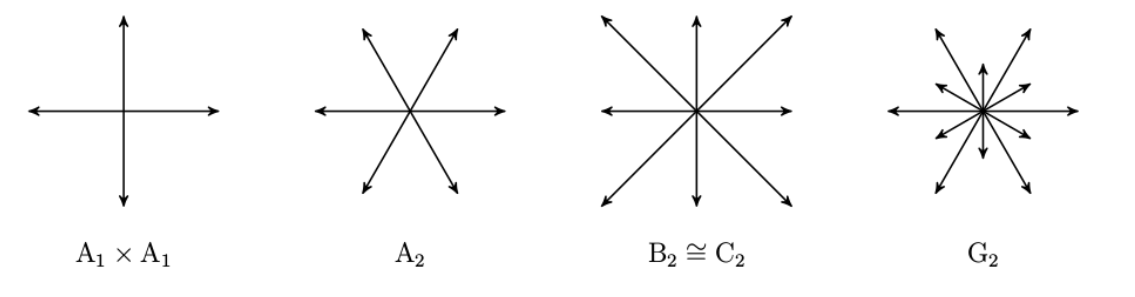
\includegraphics[width=0.9\textwidth]{img/root_systems}
\end{center}

\(\mathcal{W}(A_1 \times A_1) = \mathbb{Z}_2 \times \mathbb{Z}_2\) 

\(\mathcal{W} (A_2) = S_3\) 

\(\mathcal{W}(B_2) = D_4\) 

\(\mathcal{W}(G_2) = D_6\) 

These are the only possible cases for \(L=2\), since:
\[
    \langle \beta , \alpha  \rangle = \frac{2(\beta,\alpha)}{(\alpha,\alpha)} = \frac{2 \lVert \beta  \rVert \lVert \alpha  \rVert \cos \theta}{\lVert a \rVert \lVert a \rVert } = \frac{2 \lVert \beta  \rVert}{\lVert \alpha  \rVert} \cos \theta \in \mathbb{Z}
\]

Similarly, \(\frac{2 \lVert \alpha \rVert }{\lVert \beta  \rVert }\cos \theta \in \mathbb{Z}\). Multiplying, \(4 \cos^2 \theta \in \mathbb{Z} \implies 4\cos^2\theta = 0,1,2,3,4 \)

Thus, \(\cos \theta = 0, \pm\frac{1}{2}, \pm\frac{1}{\sqrt{2}}, \pm\frac{\sqrt{3}}{2} \implies \theta = \frac{\pi}{2}, \frac{\pi}{3}, \frac{2\pi}{3}, \frac{\pi}{4}, \frac{3\pi}{4}, \frac{\pi}{6}, \frac{5\pi}{6}\).

\begin{table}[H]
    \centering
    \begin{tabular}{c|c|c|c}
        \toprule
            \(\langle \alpha , \beta \rangle \) & \(\langle \beta , \alpha \rangle \)  & \(\theta\) &  \(\lVert \beta  \rVert ^2 / \lVert \alpha \rVert ^2\)  \\
        \midrule
            0 & 0 & \(\frac{\pi}{2}\) & undefined \\
            1 & 1 & \(\frac{\pi}{3}\) & 1  \\
            -1 & -1 & \(\frac{2\pi}{3}\) & 1 \\
            1 & 2 & \(\frac{\pi}{4}\) & 2 \\
            -1 & -2 & \(\frac{3\pi}{4}\) & 2  \\
            1 & 3 & \(\frac{\pi}{6}\)  & 3 \\
            -1 & -3 & \(\frac{5\pi}{6}\) & 3 \\
        \bottomrule
    \end{tabular}
    \caption{Angle Root System}
    \label{tab:rootsystable}
\end{table}

\begin{lemma}
    Suppose \(\alpha ,\beta \) are non-proportional root.
    
    If \((\alpha ,\beta) > 0\) then \(\alpha  - \beta \) is a root.

    If \((\alpha ,\beta ) < 0\) then \(\alpha + \beta \) is a root.

\end{lemma}

\begin{proof}
    \(\langle \alpha ,\beta  \rangle = 1 \implies \sigma_\beta (\alpha) = \alpha - 1\beta = \alpha - \beta  \in \Phi\) 

    If \(\langle \beta ,\alpha  \rangle = 1\) then \(\sigma_\alpha(\beta) = \beta - 1\alpha = \beta -\alpha \in \Phi\).
    
    \(\sigma_{\beta - \alpha}(\beta - \alpha) = (\beta - \alpha) - \langle \beta -\alpha , \beta -\alpha  \rangle (\beta -\alpha ) = \alpha - \beta \in \Phi\) 
\end{proof}

\section{Thursday, 10/3/2024, Simple Roots by Zoia}

A root system \(\Phi\) of rank \(l\), \(E\)-Euclidean Space, \(\mathcal{W}\) is the Weyl Group.

\begin{definition}
    A subset \(\Delta\) of \(\Phi\) is called a \underline{base} if:

    \begin{enumerate}[label=B\arabic*)]
        \item \(\Delta\) is a basis of \(E\) [\(\vert \Delta \vert = l\)];
        \item \(\forall \beta \in \Phi , \beta = \sum_{\alpha \in \Delta} k_\alpha \cdot \alpha\), the expression is unique with \(k_\alpha\) being integers and \(k_\alpha\) are either all non-negative or all non-positive. 
    \end{enumerate} 
\end{definition}

\begin{definition}
    The roots from \(\Delta\) are \underline{simple roots}.
\end{definition}

\begin{definition}
    The \underline{height} of a root \(\beta\) [relative to the base \(\Delta\)] is:

    \[
        \operatorname{ht} (\beta) = \sum_{\alpha \in \Delta} k_\alpha
    \]
\end{definition}

\begin{definition}
    We have \underline{positive roots} \(\Phi^+\) and negative roots \(\Phi^-\) from the sign of \(k_\alpha\). Furthermore \(\Phi^- = - \Phi^+\).

    Also, we define:

    \[
        \Phi^+(\gamma) = \{ \alpha \in \Phi \mid (\gamma , \alpha) > 0 \}
    \]
\end{definition}


\begin{definition}
    \(\gamma \in E\) is regular if:

    \[
        \gamma \in E \setminus \bigcup_{\alpha \in \Phi}^{} P_\alpha
    \]

    Otherwise it is called singular.

    Recall that \(P_\alpha =\{ \beta \in E \mid (\alpha ,\beta) = 0 \}\)
\end{definition}

\begin{definition}
    \(\alpha \in \Phi^+(\gamma)\) is \underline{decomposable} if \(\alpha = \beta_1 + \beta_2\) with \(\beta_1, \beta_2 \in \Phi^+(\gamma)\). 
    
    \(\alpha\) is \underline{indecomposable} otherwise.
\end{definition}

\begin{definition}
    We define \(\Delta (\gamma)\) to be the set of all indecomposable roots in \(\Phi^+(\gamma)\).
\end{definition}

\begin{theorem}
    Any root system \(\Phi\) has a base. Let \(\gamma \in E\) be a \underline{regular}.

    Then, the set \(\Delta (\gamma)\) of all the indecomposable roots in \(\Phi^+(\gamma)\) is a base of \(\Phi\). 

    Conversely, every base of \(\Phi\) is of the form \(\Delta(\gamma)\) for some \(\gamma\).
\end{theorem}

\begin{proof}
    We follow the following steps.
    
    \underline{Step 1}: Each root in \(\Phi^+(\gamma)\) is a non-negative \(\mathbb{Z}\)-linear combination of \(\Delta(\gamma)\). 

    \underline{Step 2}: If \(\alpha , \beta \in \Delta (\gamma)\) then \((\alpha , \beta) \leq 0\) unless \(\alpha = \beta\). 

    \underline{Step 3}: \(\Delta (\gamma)\) is a linearly independent set.

    \underline{Step 4}: \(\Delta (\gamma)\) is a base of \(\Phi\). 

    \underline{Step 5}: Each base \(\Delta\) of \(\Phi\) has the form \(\Delta (\gamma)\) for some regular \(\gamma \in E\). 

    \underline{Proof of Step 1}: Suppose otherwise. Then \(\exists \alpha \in \Phi^+(\gamma)\) that cannot be expessed as a non-negative \(\mathbb{Z}\) linear combination of \(\Delta (\gamma)\).

    We can have multiple such \(\alpha \)'s. We pick the \(\alpha\) with the smallest \((\gamma , \alpha)\).

    Note that \(\alpha \notin \Delta (\gamma)\), since if \(\alpha \in \Delta (\gamma)\) then \(\alpha = 1\cdot \alpha\), which violates the assumption. 

    Thus, \(\alpha\) can be written as sum of two elements in \(\Phi^+(\gamma)\). Suppose \(\alpha = \beta_1 + \beta_2\) so that \(\beta_1, \beta_2 \in \Phi^+(\gamma)\). Then, \((\gamma , \alpha) = (\gamma , \beta_1) + (\gamma, \beta_2)\). Due to the minimality of \((\gamma ,\alpha)\), they are both non-negative \(\mathbb{Z}\)-linear conbination of \(\Delta (\gamma)\) which means so is \(\alpha\), a contradiction.

    \underline{Proof of Step 2}: Suppose otherwise. Then, \((\alpha , \beta) > 0\). \(\beta\) cannot be \(-\alpha\), thus \(\alpha - \beta\) is a root. Then either \(\alpha - \beta\) or \(\beta - \alpha\) is in \(\Phi^+(\gamma)\). WLOG \(\alpha - \beta \in \Phi^+(\gamma)\). Then \(\alpha  = \beta + (\alpha - \beta)\). Then \(\alpha\) is decomposable, which is a contradiction since \(\Delta (\gamma)\) consists of all indecomposable roots.

    \underline{Proof of Step 3}: Suppose \(\sum_{\alpha \in \Delta (\gamma), r_\alpha \in \mathbb{R}} r_\alpha \cdot \alpha = 0\). \(r_\alpha\) can be positive or negative. We redistribute so that both sides have positive coefficient:

    \[
        \varepsilon := \sum_\alpha s_\alpha \alpha = \sum_\beta t_\beta \beta
    \]

    Then, 

    \[
        0 \leq (\varepsilon , \varepsilon) = \sum_{\alpha , \beta} \underbrace{s_\alpha t_\beta}_{\geq 0} \underbrace{(\alpha , \beta)}_{\leq 0} \leq 0 
    \]

    Thus, \(\varepsilon = 0\). Now,

    \[
        0 = (\gamma , \varepsilon) = \sum_{\alpha} \underbrace{s_\alpha}_{\geq 0} \underbrace{(\gamma,\alpha)}_{>0} \geq 0 
    \]

    Thus, \(s_\alpha = 0\) for all \(\alpha\in \Delta(\gamma)\). This implies linear independence.
    
    \underline{Proof of Step 4}: Note that \(\Phi = \Phi^+(\gamma) \cup - \Phi^+(\gamma)\). 

    B2 is satisfied because of Step 1.

    Then \(\Delta (\gamma)\) spans \(E\). Step 3 implies \(\Delta (\gamma)\) is a basis of \(E\). Thus we have B1.

    \underline{Proof of Step 5}: Given \(\Delta\), we select \(\gamma \in E : (\alpha , \gamma)> 0 \forall \alpha \in \Delta\). B2 \(\implies \gamma\) is regular and \(\Phi^+ \subseteq \Phi^+(\gamma)\). Also, \(\Phi^- \subseteq - \Phi^+(\gamma)\). 

    Therefore, \(\Phi^+ = \Phi^+(\gamma)\). \(\Delta\) consists of indecomposable elements, that is \(\Delta \subseteq \Delta (\gamma)\).

    Coordinates are equal, therefore \(\Delta = \Delta (\gamma)\).

\end{proof}

\begin{definition}
    [Weyl Chambers]
    The connected components of \(E \setminus \bigcup_{\alpha \in \Phi}^{} P_\alpha\) are called the (open) Weyl Chambers of \(E\).
    
    The fundamental Weyl chamber associated to \(\gamma\) is the open Weyl chamber containing \(\gamma\). It is denoted by \(\mathcal{C}(\gamma)\).
    
    Furthermore, \(C(\gamma) = C(\gamma ^{\prime})\) implies \(\gamma\) and \(\gamma ^{\prime} \) are on the same side of each hyperplane \(P_\alpha\). This also means \(\Delta (\gamma) = \Delta (\gamma ^{\prime} )\), so the Weyl chambers are in 1-1 correspondence with the bases.
\end{definition}

For example: here is an open Weyl Chamber for \(A_2\):

\begin{center}
    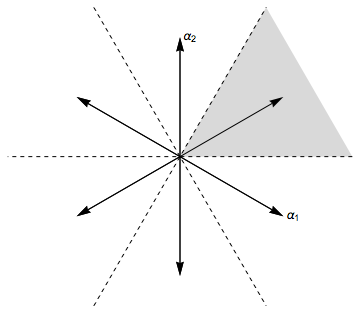
\includegraphics[width=0.5\textwidth]{img/Weyl_chambers_for_A2}

    \(\mathcal{C}(\Delta)\)-fundamental Weyl chamber relative to the base \(\{ \alpha_1, \alpha_2 \}\). 
\end{center}

The Weyl group acts on the Weyl chambers by \(\sigma (\mathcal{C}(\gamma)) = \mathcal{C}(\sigma(\gamma))\). 

If \(\sigma \in \mathcal{W}\) and \(\gamma\) is regular.

Also, \(\mathcal{W}\) permutes bases. \(\sigma\) sends \(\Delta\) to \(\sigma(\Delta)\) which is another base.

Since \(\sigma(\Delta (\gamma)) = \Delta (\sigma (\gamma))\) because \((\sigma \gamma , \sigma \alpha ) = (\gamma , \alpha)\).

\section{Thursday, 10/17/2024, Weyl Group by Zoia}

\begin{lemma}
    Let \(\alpha\) be simple. Then \(\sigma_\alpha\) permutes the positive roots other than \(\alpha\).
\end{lemma}

\begin{corollary}
    Set \(\delta = \frac{1}{2} \sum_{\beta \prec 0} \beta\). Then,

    \[
        \sigma_\alpha (\delta) = \delta - \alpha \,\forall \alpha \in \Delta
    \]
\end{corollary}

\begin{lemma}
    Let \(\alpha_1, \cdots , \alpha_n \in \Delta\) [not necessarily distinct]. Write \(\sigma_i \coloneqq \sigma_{\alpha_i}\). If \(\sigma_1 , \cdots , \sigma_{t-1}(\alpha_t)\) is negative, then
    
    \[
        \exists s : 1 \leq s < t:\, \sigma_1 \cdots  \sigma_t = \sigma_1 \cdots \sigma_{s-1} \sigma_{s+1}\cdots \sigma _{t-1}
    \]


\end{lemma}

\begin{corollary}
    If \(\sigma = \sigma_1 \cdots \sigma_t\) is an exp for \(\sigma \in \mathcal{W}\), \(t\) is as small as possible theen \(\sigma(\alpha_t) \prec 0\).
\end{corollary}

\begin{proof}
    Suppose \(\sigma(\alpha_t) > 0\). Then,

    \[
        \underbrace{\sigma_1 \cdots \sigma_t}_{t \text{ factors}} = \underbrace{\sigma_1 \cdots \sigma_{s-1}\sigma_{s+1}\cdots \sigma_{t-1}}_{t-2 \text{ factors}}
    \]

    which contradicts minimality.
\end{proof}

\subsection*{The Weyl Group}

\begin{definition}
    \(\mathcal{W}\) is the subgroup of \(GL(E)\) generated by the reflection \((\sigma_\alpha)_{\alpha \in \Phi}\).
\end{definition}

\begin{theorem}
    Let \(\Delta\) be a base of \(\Phi\).

    \begin{enumerate}[label=\alph*)]
        \item If \(\gamma \in E\), \underline{\(\gamma\) is regular}, \(\exists \sigma \in \mathcal{W} : (\sigma(\gamma), \alpha) > 0 \, \forall \alpha \in \Delta\).
        \item If \(\Delta^{\prime}\) is another base of \(\Phi\), then \(\sigma(\Delta^{\prime}) = \Delta\) for some \(\sigma\in \mathcal{W}\).
        \item If \(\alpha\) is any root \(\implies \exists \sigma \in \mathcal{W} : \sigma(\alpha)\in \Delta\).
        \item \(\mathcal{W}\) generated by \(\sigma_\alpha \,(\alpha\in \Delta)\).
        \item If \(\sigma(\Delta)=\Delta, \sigma \in \mathcal{W}\) then \(\sigma = \operatorname{id}\). 
    \end{enumerate} 
\end{theorem}

\begin{proof}
    We consider the subgroup \(\mathcal{W}^{\prime}\)  generated by \(\sigma_\alpha( \alpha \in \Delta)\).

    For a, b, c we prove the theorem for \(\mathcal{W}^{\prime}\) and for d, e we prove that \(\mathcal{W}^{\prime} = \mathcal{W}\).

    a)

    \[
        \delta \coloneqq \frac{1}{2} \sum_{\alpha \prec 0} \alpha 
    \]

    Choose \(\sigma \in \mathcal{W}^{\prime}\) such that \((\sigma(\gamma), \delta)\) is as big as possible.

    If \(\alpha\) is simple then \(\sigma_\alpha \sigma \in \mathcal{W} ^{\prime} \implies (\sigma(\gamma), \delta) \geq (\sigma_\alpha \sigma(\gamma),\delta) = (\sigma(\gamma), \sigma_\alpha(\delta))=(\sigma(\gamma), \delta -\alpha) = (\sigma(\gamma),\delta) - (\sigma(\gamma),\alpha)\).

    Therefore, \((\sigma(\gamma),\alpha)\geq 0\).

    Furthermore, \((\sigma(\gamma),\alpha)\neq 0\) so we have strict inequality. Therefore,

    \[
        \forall \alpha \in \Delta, (\sigma(\gamma), \alpha) > 0
    \]

    Therefore, \(\sigma(\gamma)\) is in the fundamental Weyl chamber of \(\Delta\) and \(\sigma\) sends \(\mathfrak{C}(\gamma)\) to \(\mathfrak{C}(\Delta)\).

    b) Since \(\mathcal{W}^{\prime}\) permutes the Weyl chambers by \(a\), it also permutes the bases of \(\Phi\).

    c) Hyperplanes \(P_\beta\, (\beta \neq \pm \alpha)\) are distinct from hyperplane \(P_\alpha \implies \exists \gamma: \gamma \in P_\alpha, \gamma \notin P_\beta\). Lets choose \(\gamma^{\prime}\) so that \(\gamma^{\prime}\) is close to \(\gamma\) such that \((\gamma ^{\prime} , \alpha) = \varepsilon > 0\) while \(\vert (\gamma^{\prime} , \beta) \vert > \varepsilon\) for any \(\beta \neq \pm \alpha\).

\end{proof}

\end{document}